
%(BEGIN_QUESTION)
% Copyright 2015, Tony R. Kuphaldt, released under the Creative Commons Attribution License (v 1.0)
% This means you may do almost anything with this work of mine, so long as you give me proper credit

{\it Weighfeeders} are conveyor belts equipped with weight sensors (load cells) to measure the weight of material on a section of the belt, and variable-speed motor drives to adjust the rate at which the belts feed material into a process.  When different solid materials are mixed together to make a blend, the weighfeeders must be connected together in a {\it ratio} configuration to maintain the desired proportion(s):

$$\includegraphics[width=15.5cm]{i01734x01.eps}$$

This particular system mixes salt, yeast, and flour together to make dry bread mix in a large factory.  The ``hand controller'' is nothing more than an operator station where a person can set a voltage signal value, in this case to be sent to a series of multiplier relays (QY) to tell each variable-speed motor drive how fast to turn.

Like many variable-speed motor drives, these units accept a 0 to 10 volt DC speed signal as an alternative to the standard 4-20 mA DC signal used in loop-powered instrumentation.  This makes the multiplier relays (QY) nothing more than potentiometers:

$$\includegraphics[width=15.5cm]{i01734x02.eps}$$

\filbreak

Given the following full-scale weighfeeder capacities (pounds per minute at full 10 volt speed signal), determine the actual ratios of salt to yeast to flour when the three potentiometers are set to the following values:

\vskip 10pt

\noindent
{\bf Weighfeeder capacities:}

\begin{itemize}
\item{} Flour weighfeeder: 100 pounds per minute
\item{} Yeast weighfeeder: 1.5 pounds per minute
\item{} Salt weighfeeder: 0.5 pounds per minute
\end{itemize}

\vskip 10pt

\noindent
{\bf Potentiometer settings:}

\begin{itemize}
\item{} $k_{flour}$ = 50\%
\item{} $k_{yeast}$ = 60\%
\item{} $k_{salt}$ = 45\%
\end{itemize}

Also, determine the total mix flow rate in pounds per minute with a hand controller setting of 70\%.

\underbar{file i01734}
%(END_QUESTION)





%(BEGIN_ANSWER)

Flour flow ratio = 97.8\% of total flow

Yeast flow ratio = 1.76\% of total flow

Salt flow ratio = 0.44\% of total flow

\vskip 10pt

Total mix flow rate at HC setting of 70\% = 35.7875 pounds per minute

%(END_ANSWER)





%(BEGIN_NOTES)

An easy way to calculate percentages is to perform a ``thought experiment'' whereby the hand controller (HIC) sends a control signal of 100\%.  This will result in the following feed rates for the three ingredients:

\begin{itemize}
\item{} 50 lbs/min of flour
\item{} 0.9 lbs/min of yeast
\item{} 0.225 lbs/min of salt
\end{itemize}

Total flow into the mixer will therefore be 51.125 lbs/min.  This yields the following ingredient ratios:

\begin{itemize}
\item{} 50 lbs/min $\div$ 51.125 lbs/min = 97.7995\%
\item{} 0.9 lbs/min of yeast $\div$ 51.125 lbs/min = 1.76039\%
\item{} 0.225 lbs/min of salt $\div$ 51.125 lbs/min = 0.440098\%
\end{itemize}

If the total flow rate at a hand controller setting of 100\% is 51.125 lbs/min, then the total flow rate at a hand controller setting of 70\% will be 70\% of that, or 35.79 lbs/min.

%INDEX% Control, strategies: ratio
%INDEX% Process: flour mixing

%(END_NOTES)


